%!TEX encoding = UTF8
%!TEX root =notes.tex
\chapter{Problèmes de géométrie}

\section{Projeté orthogonal}

	Dans cette section, et en mathématiques en général, les adjectifs \og orthogonal \fg \, et \og perpendiculaire \fg \, sont synonymes.
	On parlera alors de projeté orthogonal d'un point sur une droite lorsque les droites engendrées sont perpendiculaires.

\dfn{Projeté orthogonal}{
	Le \emph{projeté orthogonal} d'un point $M$ sur une droite $(d)$ est l'\emph{unique} point $M'$ tel que les droites $(MM')$ et $(d)$ soient perpendiculaires.
}{}

\thm{Distance minimale}{
	Le point $M'$, projeté orthogonal de $M$ sur $(d)$, est l'\emph{unique} point de $(d)$ le plus proche de $M$.
	
	Autrement dit, $M'$ est l'\emph{unique} minimiseur de la distance à $M$ en restant sur $(d)$.
}{thm:proj-min}

\pf{Démonstration du théorème \ref{thm:proj-min}}{
	Considérons un autre point $P \in (d)$ sur la droite $(d)$.
	Le triangle $MPM'$ est rectangle en $M'$, et le théorème de Pythagore implique donc que
		\[ MP^2 = MM'^2 + M'P^2. \]
	Or, comme un carré est toujours positif, on a les inégalités suivantes.
		\begin{align*}
			M'P^2 &\geq 0 \\
			M'P^2 + MM'^2 &\geq MM'^2 \\
			MP^2 &\geq MM'^2
		\end{align*}
	La distance de $M$ à $P$ est donc toujours plus grande ou égale à celle de $M$ à $M'$, ce qui démontre que $M'$ minimise sa distance à $M$ en restant sur $(d)$.
	
	Pour l'unicité, remarquons que l'égalité $MP^2 = MM'^2$ n'est vraie que lorsque $M'P^2 = 0$, c'est-à-dire lorsque $P=M'$. 
	$M'$ est donc bien l'unique point de $(d)$ le plus proche de $M$.
}

\ex{Hauteur d'un triangle}{
	Pour calculer l'aire d'un triangle on crée un rectangle grâce à sa hauteur et, par symétrie, on déduit que
		\[ \text{Aire}(\text{triangle}) = \dfrac{\text{base} \cdot \text{hauteur}}2. \]
	
	\begin{center}
	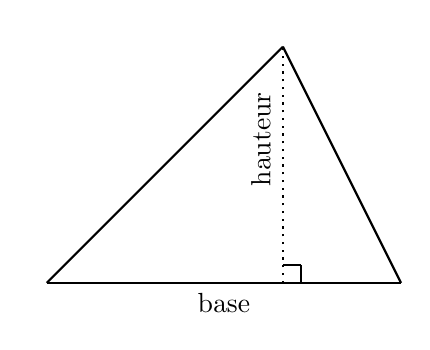
\begin{tikzpicture}[scale=1.5]
		\draw[-, thick, black] (0,0) -- (3,0) node[midway, below] {base};
		\draw[-, thick, black] (3,0) -- (2,2);
		\draw[-, thick, black] (2,2) -- (0,0);
		
		\node[black, left] at  (0,0) {};
		\node[black, below] at  (2,0) {};
		\node[black, above] at  (2,2) {};
		
		% angle droit
		\draw[-, thick, black] (2,.15)-- (2.15,.15);
		\draw[-, thick, black] (2.15,.15)-- (2.15,0);
		
		%hauteur
		\draw[-, thick, black, dotted] (2,0) -- (2,2) node[pos=.85, left=8pt, rotate=90] {hauteur};
		
	\end{tikzpicture}
	\hspace{30pt}
	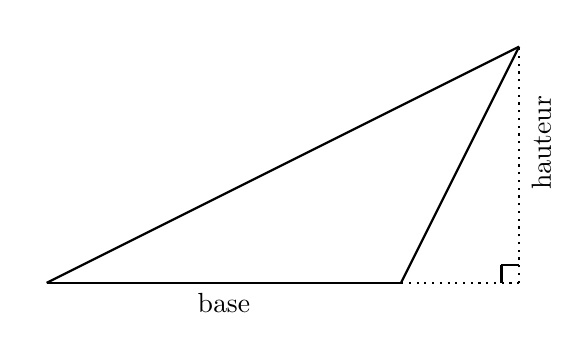
\begin{tikzpicture}[scale=1.5]
		\draw[-, thick, black] (0,0) -- (3,0) node[midway, below] {base};
		\draw[-, thick, black] (3,0) -- (4,2);
		\draw[-, thick, black] (4,2) -- (0,0);
		
		\node[black, left] at  (0,0) {};
		\node[black, below] at  (4,0) {};
		\node[black, above] at  (4,2) {};
		
		% droite base
		\draw[-, thick, black, dotted] (3,0) -- (4,0);
		
		% angle droit
		\draw[-, thick, black] (4,.15)-- (3.85,.15);
		\draw[-, thick, black] (3.85,.15)-- (3.85,0);
		
		%hauteur
		\draw[-, thick, black, dotted] (4,0) -- (4,2) node[pos=.35, right=8pt, rotate=90] {hauteur};
	\end{tikzpicture}
	\end{center}
	
	Notons que cette construction ne dépend pas de la base choisie : il faut simplement que la hauteur soit perpendiculaire à cette base, et qu'elle aille jusqu'au point culminant du triangle. 
	Ce point est nécessairement le sommet qui n'appartient pas à la base.
	
	Autrement dit, la hauteur découle du projeté orthogonal du sommet n'appartenant pas à la base sur la droite engendrée par cette base.
	
}{}

\section{Trigonométrie}

Les angles sont généralement dénotés par des lettres grecques minuscules.
	\begin{align*}
		\alpha : \text{\og alpha \fg} && \beta : \text{\og beta \fg} && \gamma : \text{\og gamma \fg} \\
		\theta : \text{\og theta \fg} &&  \delta : \text{\og delta \fg} && \omega : \text{\og omega \fg}
	\end{align*}

On rappelle les formules de trigonométrie uniquement applicables dans un triangle rectangle.
Les côtés opposé et adjacent dépendent de l'angle choisi.

	\begin{align*}
		\text{sinus} = \dfrac{\text{côté opposé}}{\text{hypoténuse}}
		&& 
		\text{cosinus} = \dfrac{\text{côté adjacent}}{\text{hypoténuse}}
		&&
		\text{tangente} = \dfrac{\text{côté opposé}}{\text{côté adjacent}}
	\end{align*}
	
	\begin{multicols}{2}
	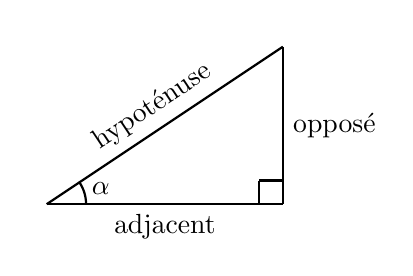
\begin{tikzpicture}[scale=1]
		\draw[-, thick, black] (0,0) -- (3,0) node[midway, below] {adjacent};
		\draw[-, thick, black] (3,0) -- (3,2) node[midway, right] {opposé};
		\draw[-, thick, black] (3,2) -- (0,0) node[midway, rotate=33.69, above]{hypoténuse};
		
		\node[black, left] at  (0,0) {};
		\node[black, below] at  (3,0) {};
		\node[black, above] at  (3,2) {};
		% angle droit
		\draw[-, thick, black] (3,.3)-- (2.7,.3);
		\draw[-, thick, black] (2.7,.3)-- (2.7,0);
		
		% angle
		\draw [black,thick,domain=0:35] plot ({.5*cos(\x)}, {.5*sin(\x)});
		\node[black, right] at  (0.45,.2) {$\alpha$};
	\end{tikzpicture}
	
	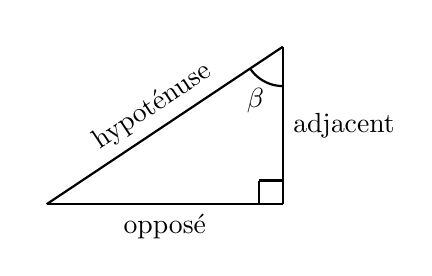
\begin{tikzpicture}[scale=1]
		\draw[-, thick, black] (0,0) -- (3,0) node[midway, below] {opposé};
		\draw[-, thick, black] (3,0) -- (3,2) node[midway, right] {adjacent};
		\draw[-, thick, black] (3,2) -- (0,0) node[midway, rotate=33.69, above]{hypoténuse};
		
		\node[black, left] at  (0,0) {};
		\node[black, below] at  (3,0) {};
		\node[black, above] at  (3,2) {};
		% angle droit
		\draw[-, thick, black] (3,.3)-- (2.7,.3);
		\draw[-, thick, black] (2.7,.3)-- (2.7,0);
		
		% angle
		\draw [black,thick,domain=215:270] plot ({3+.5*cos(\x)}, {2+.5*sin(\x)});
		\node[black, below] at  (2.65,1.6) {$\beta$};
	\end{tikzpicture}
	\end{multicols}

Moyens mnémotechniques : 
	\begin{center}
	SOH CAH TOA ou CAH SOH TOA.
	\end{center}

Remarquons immédiatement qu'on a la relation
	\begin{align*}
		\dfrac{\text{sinus}}{\text{cosinus}}
		= \dfrac{\text{opposé}}{\text{hypoténuse}} \cdot \dfrac{\text{hypoténuse}}{\text{adjacent}}
		= \dfrac{\text{opposé}}{\text{adjacent}}
		 = \text{tangente}.
	\end{align*}


\thm{}{
	Soit $\theta \in [0; 90\degree]$ un angle aigu ou droit.
	Alors 
		\[ \tan(\theta) = \dfrac{\sin(\theta)}{\cos(\theta)}. \]
}{}

\subsection{Théorème de Thalès}
	
Ces formules sont en fait une conséquence du théorème de Thalès : en connaissant deux angles et un côté d'un triangle, on peut l'agrandir ou le rapetisser pour maintenir les proportions et les angles et se ramener à un triangle rectangle étalon d'hypoténuse de longueur $1$.

	\begin{center}
	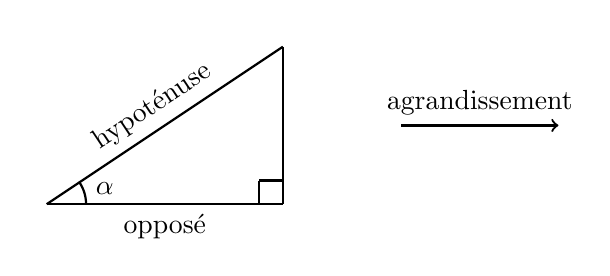
\begin{tikzpicture}[scale=1]
		\draw[-, thick, black] (0,0) -- (3,0) node[midway, below] {opposé};
		\draw[-, thick, black] (3,0) -- (3,2);
		\draw[-, thick, black] (3,2) -- (0,0) node[midway, rotate=33.69, above]{hypoténuse};
		
		\node[black, left] at  (0,0) {};
		\node[black, below] at  (3,0) {};
		\node[black, above] at  (3,2) {};
		% angle droit
		\draw[-, thick, black] (3,.3)-- (2.7,.3);
		\draw[-, thick, black] (2.7,.3)-- (2.7,0);
		
		% angle
		\draw [black,thick,domain=0:35] plot ({.5*cos(\x)}, {.5*sin(\x)});
		\node[black, right] at  (0.5,.2) {$\alpha$};
		
		% %
		
		\draw[->, thick, black] (4.5,1) -- (6.5,1) node[midway, above]{agrandissement};
		
	\end{tikzpicture}
	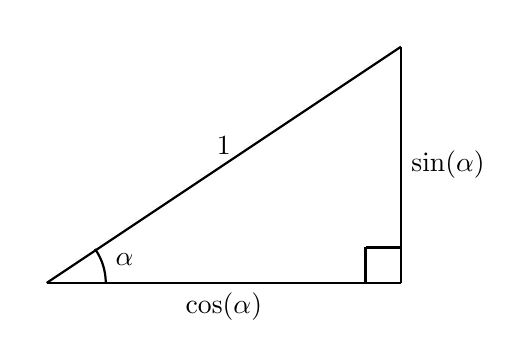
\begin{tikzpicture}[scale=1.5]
		\draw[-, thick, black] (0,0) -- (3,0) node[midway, below] {$\cos(\alpha)$};
		\draw[-, thick, black] (3,0) -- (3,2)node[midway, right] {$\sin(\alpha)$};
		\draw[-, thick, black] (3,2) -- (0,0) node[midway, above]{1};
		
		\node[black, left] at  (0,0) {};
		\node[black, below] at  (3,0) {};
		\node[black, above] at  (3,2) {};
		% angle droit
		\draw[-, thick, black] (3,.3)-- (2.7,.3);
		\draw[-, thick, black] (2.7,.3)-- (2.7,0);
		
		% angle
		\draw [black,thick,domain=0:35] plot ({.5*cos(\x)}, {.5*sin(\x)});
		\node[black, right] at  (0.5,.2) {$\alpha$};
		
	\end{tikzpicture}
	\end{center}

En effet, les deux triangles ci-dessus sont semblables (on obtient l'un en (dé)zoomant l'autre), et en \emph{définissant} les longueur des côtés du deuxième par $\cos(\alpha)$ et $\sin(\alpha)$, le théorème de Thalès nous donne, par exemple,
	\[ \dfrac{\cos(\alpha)}{1} = \dfrac{\text{opposé}}{\text{hypoténuse}}. \]

En conclusion, le cosinus, le sinus, et la tangente sont donc en fait une banque de données de longueurs de côtés d'un triangle particulier qu'on a mesuré à l'avance.
Certaines formules mathématiques permettent de calculer exactement ces valeurs, mais en général elle sont approximatives (mais aussi précises qu'on le souhaite !) et il n'existe pas de formule compacte pour les exprimer.

\subsection{Quart de cercle trigonométrique}

Considérons, dans le quadrant supérieur-droit d'un repère d'origine $O$, un quart de cercle de rayon $1$.
On choisit un angle $\theta \in [0, 90\degree]$, et on nomme le point $P$ du quart de cercle tel que l'angle entre $(OP)$ et l'axe des abscisse soit $\theta$.

	\begin{center}
	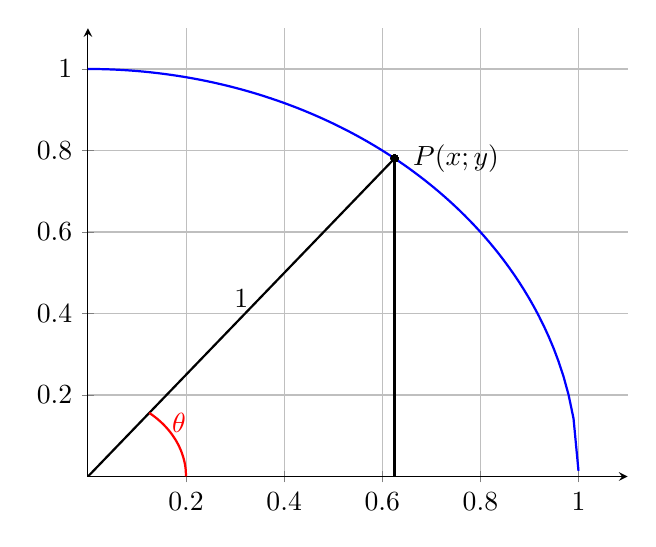
\begin{tikzpicture}[>=stealth, scale=1]
		\begin{axis}[xmin = 0, xmax=1.1, ymin=0, ymax=1.1, axis x line=middle, axis y line=middle, axis line style=->, grid=both]
			\addplot[no marks, blue, -, thick] expression[domain=0:1, samples=100]{sqrt(1-x^2)};
			\addplot[black, mark=*, mark size = 1, thick] (0.625, 0.7805) node[right=3pt] {$P(x;y)$};
			
			
			\addplot[no marks, black, -, thick] expression[domain=0:0.625, samples=2]{0.7805/0.625*x}
			node[midway, above=]{$1$};
			
			\addplot[no marks, red, -, thick] expression[domain=0.125:.2, samples=100]{sqrt(.04-x^2)}
			node[right, pos=.2] {$\theta$};
			
			\draw[black, thick] (axis cs:0.625, 0) -- (axis cs:0.625,0.7805);
		\end{axis}
	\end{tikzpicture}
	\end{center}

Le triangle rectangle ainsi créé est d'hypoténuse $1$ et vérifie donc les propriétés du triangle étalon considéré dans la section précédente.
On a donc, par définition,
	\begin{align*}
		x = \cos(\theta), && \text{ et } && y = \sin(\theta).
	\end{align*}
Si on a pas peur des raisonnements circulaires, on peut revérifier les égalités avec les formules apprises.
Par exemple,
	\[
		\cos(\theta) = \dfrac{\text{adjacent}}{\text{hypoténuse}} = \dfrac{x}{1}.
	\]
En conclusion, les coordonnées du point $P$ sont exactement
	\[ P = (x ; y) = \left( \cos(\theta) ; \sin(\theta) \right). \]
Dans ce contexte, on déduit naturellement le théorème suivant, après une introductions aux notations.

\nt{
	Comme il est assez fastidieux d'écrire
		\[ \left(\cos\left(\theta\right)\right)^2, \]
	on optera pour la notation plus allégée suivante.
		\[ \left(\cos\left(\theta\right)\right)^2 = \cos^2 (\theta). \]
}{}

\thm{}{
	Soit $\theta \in [0; 90\degree]$ un angle aigu ou droit.
	Alors, 
		\begin{align*}
			0 \leq \cos(\theta) \leq 1, &&
			0 \leq \sin(\theta) \leq 1,
		\end{align*}
	et
		\begin{gather*}
			\cos^2(\theta) + \sin^2(\theta) = 1.
		\end{gather*}
}{}


\section{Manipulations des racines carrées}



